\documentclass[11pt]{article}
\usepackage{graphics,epsfig,amsmath,amssymb}
\usepackage{epsf}
\usepackage{boxedminipage}
\usepackage{fullpage}
\usepackage{fancyheadings}
\usepackage{times}
\usepackage{amsmath}
\usepackage{ifthen}
\usepackage{url}
%\usepackage{pseudocode}
\usepackage{psfrag}
\pagestyle{fancy}

\setlength{\topmargin}{.2in}
\setlength{\parindent}{0in}
\setlength{\parskip}{.15in}
\setlength{\footskip}{0.1in}

\newcounter{pctr}
\stepcounter{pctr}

\newcounter{partctr}

\newcommand{\ie}{{\em i.e.}}
\newcommand{\eg}{{\em e.g.}}

\newcommand{\ch}{\item {\bf True~~/~~False~~}}
\newcommand{\tfnote}{\probnote{Circle True or False for each choice.}}
\newcommand{\allapply}{\probnote{Circle ALL that apply}}
\newcommand{\bestanswer}{\probnote{Circle the BEST answer}}
\newcommand{\ansbelow}{\probnote{Answer legibly in the space below.}}

\renewcommand{\thesection}{{\bf\Roman{section}}}
\renewcommand{\theenumi}{{\bf\Alph{enumi}.}}
\renewcommand{\labelenumi}{{\bf\Alph{enumi}.}}

\newcommand{\setversion}[1]{\def\version{#1}}
\setversion{answers}

\ifthenelse{\equal{\version}{answers}}{
    \newcommand{\sols}[1]{#1}
} {
    \newcommand{\sols}[1]{}
}


\newcounter{answer}
\newenvironment{answer}[1][\relax]{\refstepcounter{answer}\begin{list}%
 {}{\leftmargin 0pt\rightmargin 0pt\labelsep 3pt\parsep 0pt%
 \setlength{\listparindent}{\parindent}}
    \item {\bf Answer \theanswer #1}\
    }{\hspace*{\fill}$\blacksquare$\end{list}} 



% uses these macros to delimit problems
\newcommand\prob[1]%
  {\begin{itemize}\item[]%
   \vspace{.2in}{\bf\thepctr. ~[#1~ points]:}\stepcounter{pctr}}
\newcommand\eprob{\end{itemize}}
\newcommand\probnote[1]%
  {\\\begin{tabular}{cr} \hspace{3in} & {\bf (#1)} \\ \end{tabular}}

% headers/footers
\lhead[\fancyplain{}{\bf Page \thepage ~of \pageref{lastpage}}]%
      {CS 6250 Fall 2010, Quiz 2}
\lfoot[{\bf Initials: }]%
      {{\bf Initials: }}
\rhead[CS 6250 Fall 2010, Quiz 2]%
      {\fancyplain{}{\bf Page \thepage ~of \pageref{lastpage}}}
\cfoot{}
\setlength{\headrulewidth}{0in}
\setlength{\headsep}{.3in}

 % Compact itemize and enumerate.  Note that they use the same counters and
% symbols as the usual itemize and enumerate environments.
\def\compactify{\itemsep=0pt \topsep=0pt \partopsep=0pt \parsep=0pt}
\let\latexusecounter=\usecounter
\newenvironment{CompactItemize}
  {\def\usecounter{\compactify\latexusecounter}
   \begin{itemize}}
  {\end{itemize}\let\usecounter=\latexusecounter}
\newenvironment{CompactEnumerate}
  {\def\usecounter{\compactify\latexusecounter}
   \begin{enumerate}}
  {\end{enumerate}\let\usecounter=\latexusecounter}

\begin{document}
\cfoot{}
\pagestyle{empty}
\begin{center}
\begin{tabular}{lr}
\resizebox{1in}{!}{
\includegraphics{GT}}
&
\parbox{4in}{
    {\Large\it College of Computing} \\ \\
    {\LARGE\sf Georgia Institute of Technology} 
}
%
\end{tabular}
\end{center}

\begin{center}
{\Large{\bf CS 6250: Computer Networking: Fall 2010} \\
 \vspace{.15in} \Huge{\bf Quiz II}} 
\vspace{.2in}

% this is the box on the first page with overall quiz information
\begin{boxedminipage}[h]{6in}
There are \underline{14 questions} and
  \underline{\pageref{lastpage} pages} in this quiz booklet (including
  this page).  Answer each question according to the instructions given.
  You have {\bf 85 minutes} to answer the questions.

%\vspace{.1in} The last page is an easy question.  {\em Rip this
%page off of your exam for five bonus points.}  Turn it in anonymously if
%you like.


\vspace{.1in} 
If you find a question ambiguous, write down any
assumptions you make.  {\bf Be neat and legible.}  If I can't
understand your answer, I can't give you credit!  There are three pretty
challenging questions (clearly marked); you may want to look through the
whole quiz and save those for last.

\vspace{.1in} 
Use the empty sides of this booklet if you need scratch space.  You
may also use them for answers, although you shouldn't need to.  {\em If you
do use the blank sides for answers, make sure to clearly say so!}

\vspace{.1in} 
{\bf Note well: Write your name in the space below AND your initials at the bottom of each
page of this booklet.}

\begin{center}{\bf THIS IS AN ``OPEN NOTES, OPEN PAPERS'' QUIZ.\\
NO OTHER MATERIALS, NO PHONES, NO COMPUTERS, NO LAPTOPS, NO PDAS.\\
%NO ENCRYPTED WIRELESS TRAFFIC. \\
MAKE SURE YOU'VE READ ALL THE INSTRUCTIONS ABOVE!}
\end{center}
{\em Initial here to indicate that (1)~you've read the instructions and (2)~
you agree to abide by the Georgia Tech Honor Code: }



\vspace{.05in} The last page has easy bonus questions, {\em which you can
answer outside of the allotted time}.  Rip the last page off of your
quiz for five bonus points.  Turn it in anonymously if you like (feel
free to fill it out after the quiz and give it to a TA, or take it with you).  You
won't get the five points if you don't tear off the page (this is to
make certain you've read this far ;).

\end{boxedminipage}
\end{center}
\vspace*{0.15in}
\begin{center}
{\it Do not write in the boxes below}
\end{center}

\begin{center}
\begin{tabular}{|l|l|l|l|l|l|l|l|l|} \hline \hline
{\bf 1-5 (xx/20)}& {\bf 6-10 (xx/28)}& {\bf 11-13 (xx/13)} &{\bf Bonus (xx/9)} & {\bf Total
  (xx/70)}  \\ \hline 
 & & & & \\ 
 & & & &\\ \hline \hline
\end{tabular}
\end{center}

\vspace{.1in}
{\bf\Large{Name:}}

\newpage
\pagestyle{fancy}

\section{Warmup}



\prob{4} Which of the following is true about various measurement techniques?
\allapply

\setcounter{partctr}{0}
\begin{list}{\bf\Alph{partctr}.}{\usecounter{partctr}}
\item From a flow-level trace, one cannot compute the jitter experienced
  by the flow.
\item Collecting flow statistics from a sampled packet trace may result
  in no statistics being gathered about small flows.
\item From a flow-level trace, one cannot compute the average packet
  size for each flow in the trace.
\item The ability to compute the round-trip time perceived by a client
  on one end of a TCP connection from a packet trace depends on where
  the packet trace was captured.
\item All of the above.
\end{list}
\eprob

\sols{
\begin{answer}
The answer is: (A), (B).
\end{answer}
}


\prob{4} Which of the following are true about spam filtering techniques?
\allapply

\setcounter{partctr}{0}
\begin{list}{\bf\Alph{partctr}.}{\usecounter{partctr}}
\item DNS-based blacklists are difficult to keep up-to-date because IP
  addresses of spammers keep changing.
\item It is possible to send spam from a ``spoofed'' IP address.
\item Most spam is sent from ``spoofed'' IP addresses.
\item Most spam comes from botnets.
\item None of the above.
\end{list}
\eprob

\sols{
\begin{answer}
The answer is : (A), (B), (D).  (Some folks may not circle B, but it is
technically possible with BGP route hijacking.)
\end{answer}
}

\prob{4} Which of the following is true about data-center network architectures?
\allapply
\setcounter{partctr}{0}
\begin{list}{\bf\Alph{partctr}.}{\usecounter{partctr}}
%\begin{enumerate}
\item The current Yahoo data center network design uses no IP routing.
\item The VL2 design requires modifications to the host network stack. 
\item The VL2 design relies on Valiant load balancing to spread traffic
  across the aggregation switches.
\item In Seattle, a host can discover the MAC address for a certain IP
  address by sending an ARP request.
\item All of the above.
\end{list}
\eprob

\sols{
\begin{answer}
The answer is: (B), (C), (D).
\end{answer}
}

\pagebreak
\prob{4} Which of the following is true about programmable network
software and hardware?
\allapply
\setcounter{partctr}{0}
\begin{list}{\bf\Alph{partctr}.}{\usecounter{partctr}}
\item Running a Click program in the kernel can speed up packet forwarding
  from running them in user space.
\item A RouteBricks cluster can achieve faster forwarding performance because
  packets never need to be forwarded across the PCI bus.
\item One of the major disadvantages of programming a custom data plane
  for the NetFPGA is that it is difficult to program.
\item One of the major disadvantages of programming a custom data plane
  for a Click software router is that the developer can only use the
  elements that the Click software distribution provides.
\item All of the above.
\end{list}
\eprob

\sols{
\begin{answer}
The answer is (A), (C).
\end{answer}
}


\prob{4} Which of the following is true about BGP security and route hijacking?
\allapply
\setcounter{partctr}{0}
\begin{list}{\bf\Alph{partctr}.}{\usecounter{partctr}}
%\begin{enumerate}
\item If a route is hijacked, one can determine the party that is
  responsible for the hijack by looking at the origin AS in the AS path
  (i.e., the last AS in the AS path).
\item An attacker who hijacks a route can always be discovered using
  traceroute.
\item One of the main reasons S-BGP has not been deployed is that
  deploying it slows packet forwarding rates considerably.
\item One of the main reasons S-BGP has not been deployed is that it
  requires everyone to deploy it before any AS sees any benefits.
\item None of the above
\end{list}
\eprob

\sols{
\begin{answer}
The answer is (D).
\end{answer}
}


%%%%%%%%%%%%%%%%%%%%%%%%%%%%%%%%%%%%%%%%%%%%%%%%%%%%%%%%%%%%

\newpage
\section{Potpourri}


\prob{5} Give a simple example where network tomography using end-to-end
packet probes from multiple locations can isolate a link failure.  Give
{\em two} possible reasons why binary tomography might be inaccurate in
practice.~\ansbelow 
\vspace{2in}
\eprob

\sols{
\vspace{-1.25in}
\begin{answer}
A simple example here would illustrate something as in the binary
tomography slides: For example, two end-to-end probes starting from the
same source but going to two different destinations.  If one end-to-end
probe succeeded, but the other failed, you would know that the failure
was on the link that corresponded to the failed probe, but not the
other.  (A picture here would be most illustrative.)

Binary tomography might be inaccurate in practice because failures might
be mistaken for congestion, or because measurements of the reachability
matrix may be inconsistent (e.g., due to re-routing during a failure
event). 
\end{answer}
}

\prob{4} Give an example of an {\em intra-firewall inconsistency} where
a subset of packets matched to the current rule would have been matched
by a preceding rule that took a different action.  How might such an
inconsistency arise in practice?~\ansbelow
\vspace{1.25in}
\eprob

\sols{
\vspace{-1.25in}
\begin{answer}
One example of an intra-firewall inconsistency would be a rule that
denied all packets from a $/16$ subnet, but then a later rule in the
chain that allowed all packets from a $/24$ subnet contained inside of
that original $/16$ (any such subnetting inconsistency where the smaller
subnet contradicted the actions from the earlier subnet would be
acceptable here).
\end{answer}
}

\newpage

%% \pagebreak
\prob{6} Consider the BGP routing table shown below like the one you saw
in Problem Set~2, which contains a
single route per prefix.

\begin{verbatim}
*> 8.14.0.0/19      143.215.254.25          0 2637 209 3356 46164 i
*> 8.14.0.0/20      143.215.254.25          0 2637 174 7018 46164 i
*> 8.14.16.0/20     143.215.254.25          0 2637 174 7018 46164 i
*> 8.14.38.0/24     143.215.254.25          0 2637 209 3356 53317 53317 i
*> 8.14.52.0/24     143.215.254.25          0 2637 209 3356 30016 i
*> 8.14.53.0/24     143.215.254.25          0 2637 209 3356 30016 i
*> 8.14.57.0/24     143.215.254.25          0 2637 174 33012 i
\end{verbatim}

\setcounter{partctr}{0}
\begin{list}{\bf\Alph{partctr}.}{\usecounter{partctr}}
\item List two {\em contiguous} IP prefixes in the table that are
  advertised by the same origin AS.  
\item What might be a reason that an AS advertises two contiguous
  prefixes? 
\item List two {\em overlapping} IP prefixes advertised by the same AS.  
\item What might be a reason that an AS advertises two overlapping IP
  prefixes?
\item List an AS path that uses {\em AS Path Prepending} in this table.
\item Each IP prefix in this table has only one route.  Does that imply
  that AS path prepending did not have any effect on traffic flow along
  that path?  Why or why not?
\end{list}
~\ansbelow
\eprob

\sols{
\begin{answer}
Two contiguous prefixes advertised by the same AS are 8.14.52.0/24 and
8.14.53.0/24.  One reason that an AS advertises two contiguous prefixes
would be for inbound traffic control for traffic engineering.  Two
overlapping IP prefixes advertised by the same AS are 8.14.0.0/19 and
8.14.0.0/24.  One reason that an AS might advertise two overlapping
prefixes is, again, for inbound traffic engineering.  Another possible
reason would be provider-based addressing (perhaps the AS has a
downstream customer that is advertising this prefix via both this
upstream AS, and another upstream).  This second answer should likely
only get half credit, since it is not quite feasible.  An AS that uses
AS path prepending is 53317.  AS path prepending could have had an effect
on the router that is directly upstream of this router, for example, so
it is not correct to say that AS path prepending did not have any
effect, even in this case.
\end{answer}
}


\pagebreak

\prob{5} Consider the graph below, as seen in lecture, which shows
samples of round-trip time latency for several months between an
apartment in Atlanta and Georgia Tech, over a DSL link.  The $y$ axis
shows round-trip time latencies in milliseconds.
\centering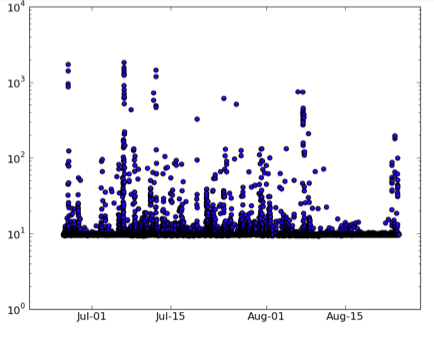
\includegraphics[width=0.75\linewidth]{rtt.png}
\setcounter{partctr}{0}
\begin{list}{\bf\Alph{partctr}.}{\usecounter{partctr}}
\item Give {\em two} reasons why the latencies might vary drastically
  over time.
\item Assume that, when latency gets very high, uploads are inducing
  congestion on the access link that is causing the additional latency.
  Also assume that the uplink speed is 1 Mega{\em bit} per second.
  Suppose also that buffering at the first hop is imposing the delay,
  and that no packets are dropped.  

  How large must the buffer on this first hop be, if packets are
  experiencing round-trip times of one second?
\item Why might access links use large buffers?
\item What is a disadvantage of using large buffers on the access link?
\end{list}
~\ansbelow
\eprob

\sols{
\begin{answer}
Latencies could vary over time due to congestion on the access link
introduced by the user's own traffic (either uploads or downloads could
cause buffering at the access link).  Latencies might also vary due to
congestion at otehr bottlenecks along the end-to-end path.

The buffer must be large enough to cause a one-second delay for some
packets on a 1 Mbps link.  So, that would be 1 Mbps times 1 second = 1
Mb.

Access links might use large buffers to help reduce packet loss.  The
disadvantage of such large buffering is that it can make it difficult to
use interactive applications, since large variances in latencies could
be introduced.  An interesting recent discussion of this phenomenon is
available here:
\url{https://gettys.wordpress.com/2010/12/06/whose-house-is-of-glasse-must-not-throw-stones-at-another/}. 
\end{answer}
}


%% \prob{4} Recall from the {\em NetPrints} paper that the system uses the
%% notion of a ``change tree'' to help users fix their network
%% configurations.  Explain how the system constructs a change tree and the
%% relationship of a change tree to a decision tree.
%% Explain one possible case where the change tree might cause a user to make
%% an inconvenient (or incorrect) change to their home network
%% ~\ansbelow
%% \vspace{1.75in}
%% \eprob

%% \sols{
%% \vspace{-1.25in}
%% \begin{answer}
%% \end{answer}
%% }


\pagebreak
\prob{8} 
Consider the following graph, which shows the flow-size distribution for
flows captured on the Georgia Tech campus network in 2007.

\centering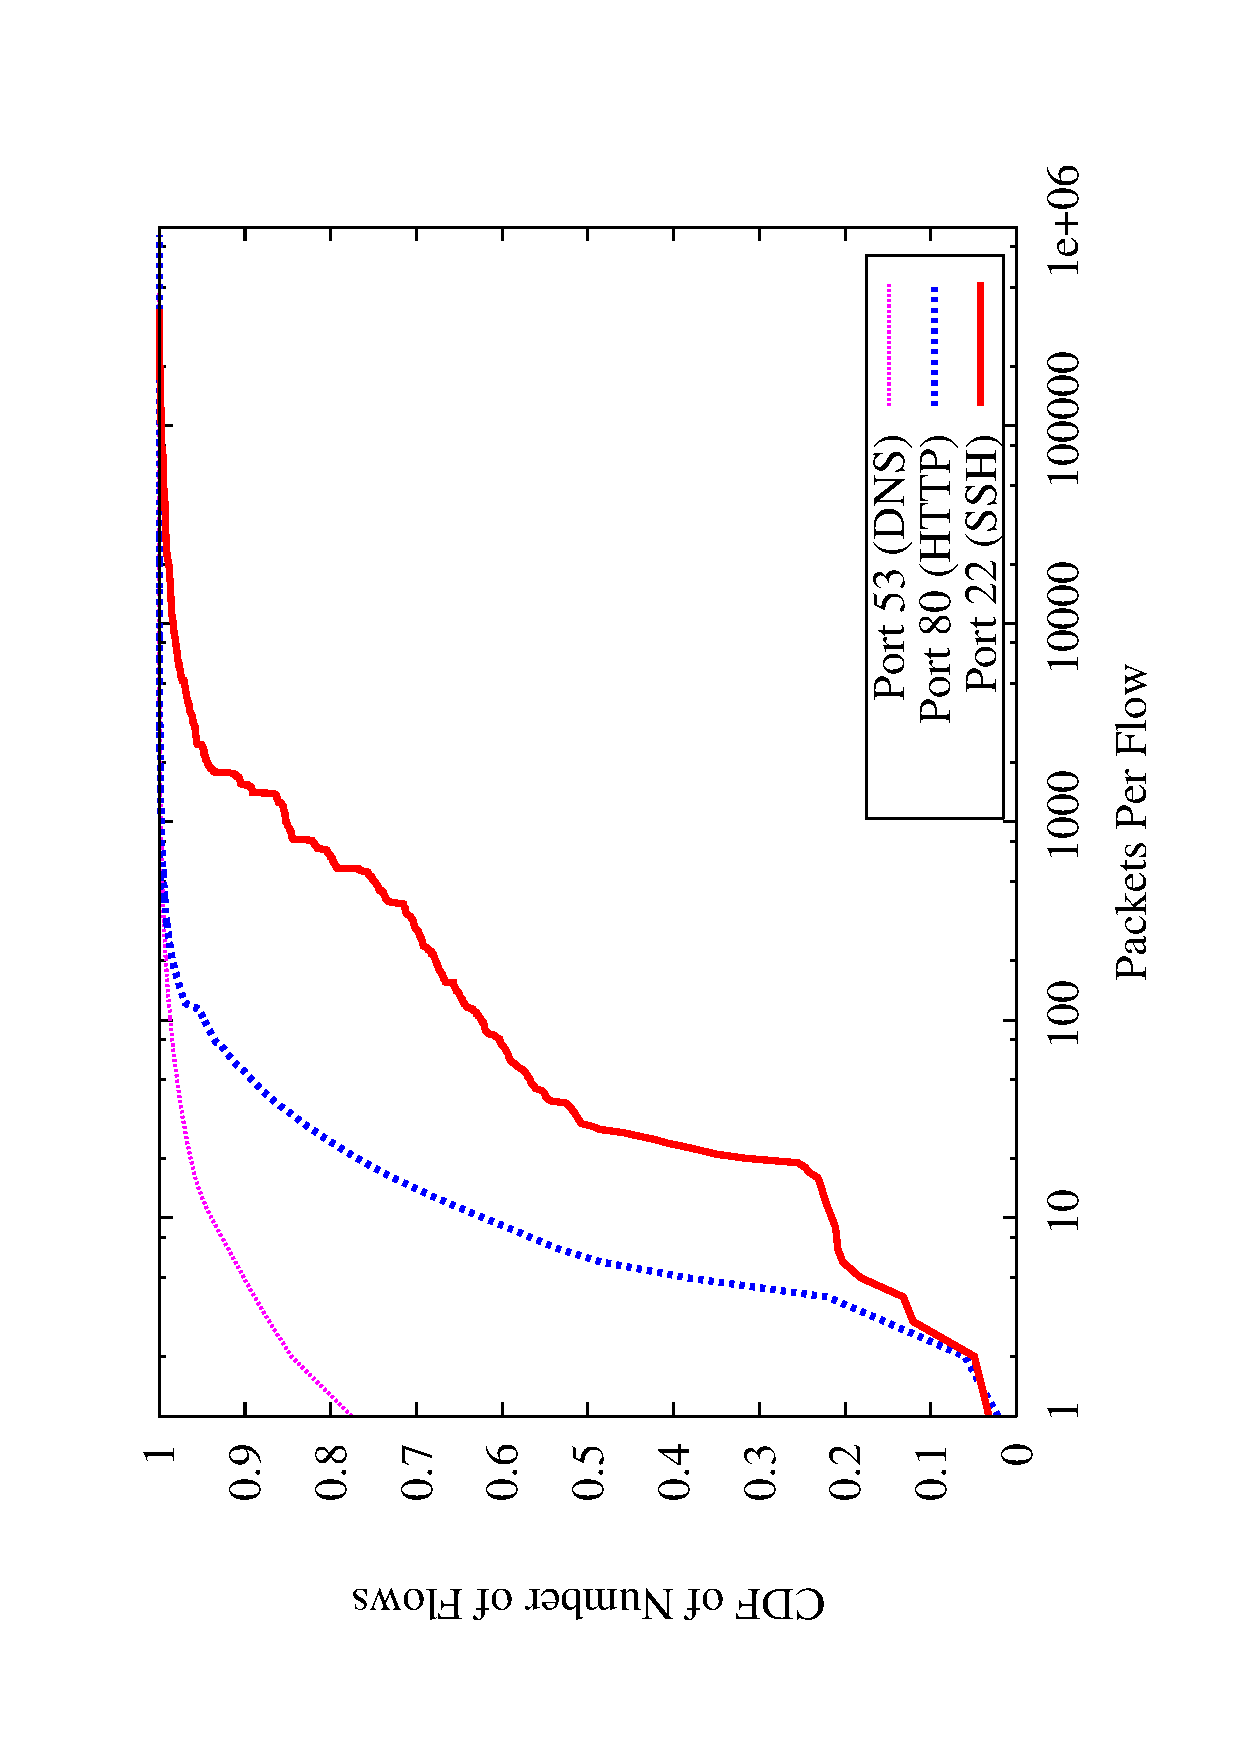
\includegraphics[width=0.5\linewidth, angle=270]{port225380stats}

\begin{verbatim}

\end{verbatim}

\setcounter{partctr}{0}
\begin{list}{\bf\Alph{partctr}.}{\usecounter{partctr}}
\item Which protocol has the smallest median number of packets per flow?
\item What is the median number of packets for the protocol you named in
  part (a)? 
\item Why are the flows for that protocol so small?
\item Which protocol has the largest number of median packets per flow?
\item Assume that this graph was generated directly from flow records
  ``dumped'' from a Cisco router, with no post processing of the flow
  records.  From the lecture on flow monitoring, list {\em two}
  potential sources of inaccuracy that this graph might have.  (In
  other words, why might the flow sizes be inaccurate?)
\end{list}

~\ansbelow 
\vspace{2in}
\eprob

\sols{
\vspace{-2in}
\begin{answer}
DNS has the smallest number of median packets per flow (one packet).
The flows are likely small for that protocol because most DNS lookups
can fit into a single packet.  ssh, on the other hand, has a larger
number of median packets per flow.  Flow sizes might be inaccurate,
particularly for ssh, because flow monitoring automatically ``dumps''
the flow records after (1) a period of ``silence'' (i.e., no packets);
(2) after a fixed period of time, on a regular basis (i.e., once every
30 minutes).  These can cause longer flows to be inadvertently broken up
into smaller flows.
\end{answer}
}

\newpage
\section{Design Question: Routing Security}

For this problem, consider the AS diagram shown below.  To indicate that
message $M$ is signed with the private key belonging to AS $i$, you may
use the notation $\{M\}_i$.

\centering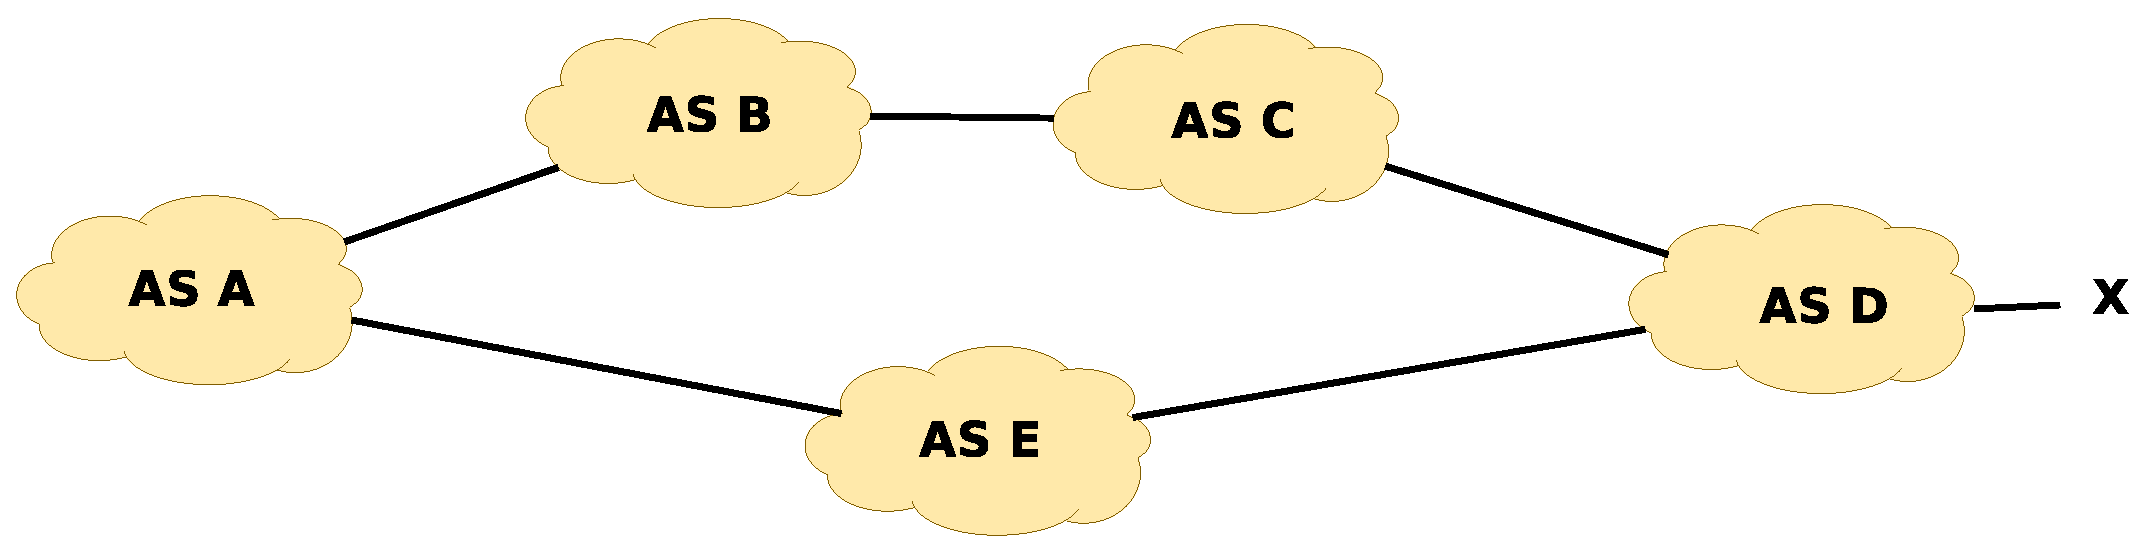
\includegraphics[width=0.75\linewidth]{ases}


\prob{4} Suppose that AS $D$ advertises a route for IP prefix $y$ to
both AS $C$ and AS $E$.  Given equal local preference settings, AS $A$
would select the route through AS $E$.  Describe an attack that AS $B$
could mount to try to ``attract'' traffic destined for IP prefix $y$.  
\vspace*{1.5in}

~\ansbelow
\eprob

\sols{
\begin{answer}
AS $B$ could remove AS $C$ from the AS path that it advertises to AS $A$
for destination $x$, effectively having AS $A$ see two AS paths of equal
length---$AED$ and $ABD$.  If it treated routes from $B$ and $E$ with
equal local preference, there is some chance that AS $A$ might start
sending more traffic through AS $B$ as a result of this ``path
shortening'' attack. 
\end{answer}
}


\prob{4} Suppose now that these ASes all deploy Secure BGP (S-BGP).
Annotate the edges of the graph below to indicate {\em all} of the
signed route attestations that each AS advertises along with the route.
Use the notation recommended above: for example, $\{X Y Z\}_W$ would
indicate that AS $W$ signed the AS path $X Y Z$ with its private key.
{\em Hint: Be careful to sign the correct AS path; be careful to defend
  against route shortening attacks.}  

\vspace*{0.5in}
\centering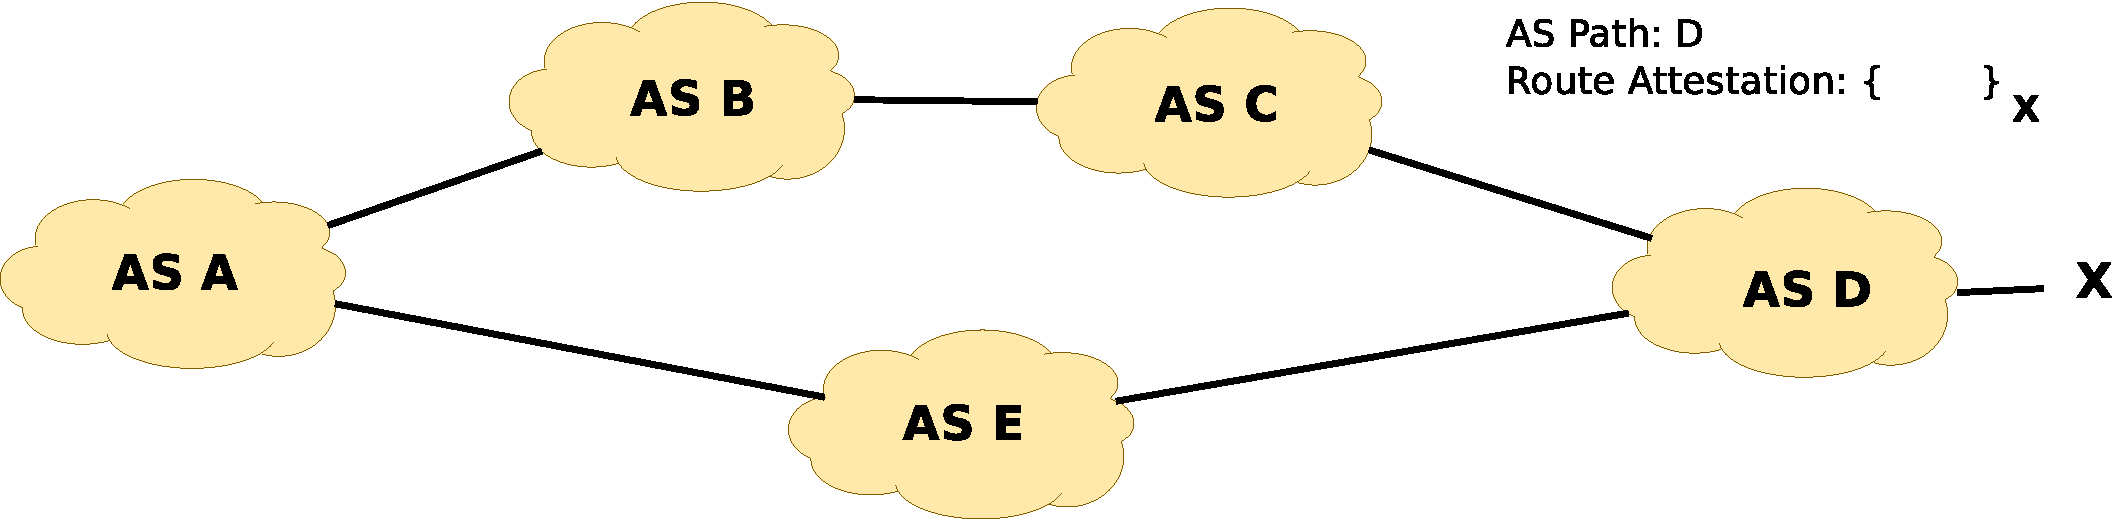
\includegraphics[width=0.9\linewidth]{ases2}

\eprob

\sols{
\begin{answer}
Between AS $D$ and AS $C$: AS Path: $D$, Route Attestation: $\{CD\}_D$\\
Between AS $C$ and AS $B$: AS Path: $D$, Route Attestation: $\{CD\}_D$,
$\{BCD\}_C$ \\
Between AS $B$ and AS $A$: AS Path: $D$, Route Attestation: $\{CD\}_D$,
$\{BCD\}_C$, $\{ABCD\}_A$ \\

Between AS $C$ and AS $D$: AS Path: $D$, Route Attestation: $\{ED\}_D$\\
Between AS $C$ and AS $D$: AS Path: $D$, Route Attestation: $\{ED\}_D$,
$\{AED\}_E$ \\
\end{answer}
}

\pagebreak
\prob{5} George Burdell notes that, if a router should happen to reboot,
it would have to sign hundreds of thousands of routes before advertising
a full routing table to its neighbor AS, and the neighbor AS would have
to verify the signatures on all of these routes.  How might you design a
scheme to speed up the process of signing and verifying advertisements
for a full routing table's worth of route advertisements?  ({\em Hint:}
Think about some things that are common across routing advertisements.)
~\ansbelow
\eprob

\sols{
\begin{answer}
One possibility might be to have a {\em cache} of route signatures for each
route attestation.  You could, for example, cache the result of each
signed route attestation, since the AS paths for the routes coming from
a neighbor would likely be the same as they were before the reboot
occurred.  

One additional consideration with this approach is that caching old
signatures could make the router vulnerable to a replay attack.  So, a
more robust solution would be to also include a timestamp with the route
attestation, to prevent replay.  (In fact, S-BGP's route attestations
already include such a timestamp.)
\end{answer}
}

\prob{9} {\em Bonus.} George also notes that S-BGP provides no mechanism
for guaranteeing the authenticity of a BGP withdrawal message.  Design a
scheme that prevents at attacker from forging a BGP withdrawal message.
Your solution need not be cryptographic.  (Feel free to use
cryptography, of course, but you could take other approaches; for
example, you could use views of the Internet routing table from multiple
vantage points.)
~\ansbelow
\eprob

\sols{
\begin{answer}
One simple approach would be to have the neighbor AS sign the BGP
withdrawal messages, but that doesn't completely work, since the
neighbor AS could actually withdraw a prefix for a network that is
downstream.  Really, you would need a scheme that allows the AS to
determine {\em who initiated the withdrawal}, and that the {\em
  withdrawal was initiated by someone who has the right to initiate that
  withdrawal}.  There's actually no good answer to this, because anyone
could initiate the withdrawal of any prefix, for a variety of reasons
(\eg, an AS might withdraw a more specific route for traffic engineering
reasons).  

Two parts to the solution that should get credit are: (1)~recognizing
that a withdrawal could be originated from anywhere, not just the
immediate AS neighbor; (2)~somehow developing a scheme that attributes
the BGP withdrawal to a particular AS ({\em not only the neighbor}).
\end{answer}
}


\label{lastpage}
\end{document}


\newpage
\section{Bonus: Anonymous Course Feedback}

{\bf This page is anonymous.}  Rip this off from your exam, and turn it
in separately if you like.  You'll get five points for simply ripping
off the last page of the exam, but I'd prefer if you fill it out and
hand it in in a separate stack.
\vspace{.5in}

What are the things you like most about the course so far?  Anything is
fair game here (topics, course structure, board technique, etc.).
\vspace{1.5in}


What are the things you like least about the course so far?  Again,
anything is fair game.
\vspace{1in}


What topics would you like to see covered?
\vspace{1in}



